\documentclass{paper}
\usepackage{hyperref}
\usepackage{datetime}
\usepackage{listings}
\usepackage{graphicx}
\usepackage{float}
\usepackage{hyphenat}
\title{Automated Continious Integration with Travis}
\newdate{date}{24}{02}{2020}
\date{\displaydate{date}}
\author{John Ghatas}

\hypersetup{
    colorlinks=true,
    linkcolor=black,
    urlcolor=blue,
    linktoc=all
}

\begin{document}
    % Page 1
    \maketitle
    \newpage
    
    % Page 2
    \tableofcontents
    \newpage

    % Page 3
    \section{Project definition}
    \paragraph{Goal}{This project was pulled from a Lynda tutorial teaching the basics of Docker, 
    the Docker container created runs an express backend using MongoDB as the database server.}

    \section{Running the application}{The first order of business was to ensure that the application
    was able to run locally before deploying it in a Docker container. To do this we ran the following commands in
    the main directory:
    \begin{lstlisting}[language=bash]
        $ npm install
        $ npm start
    \end{lstlisting}
    To start the backend locally \textbf{MongoDB} is required to have a local install. An example of the backend is shown
    in \textbf{Figure \ref{fig:backend}}
    \begin{figure}[!h]
        \centering
        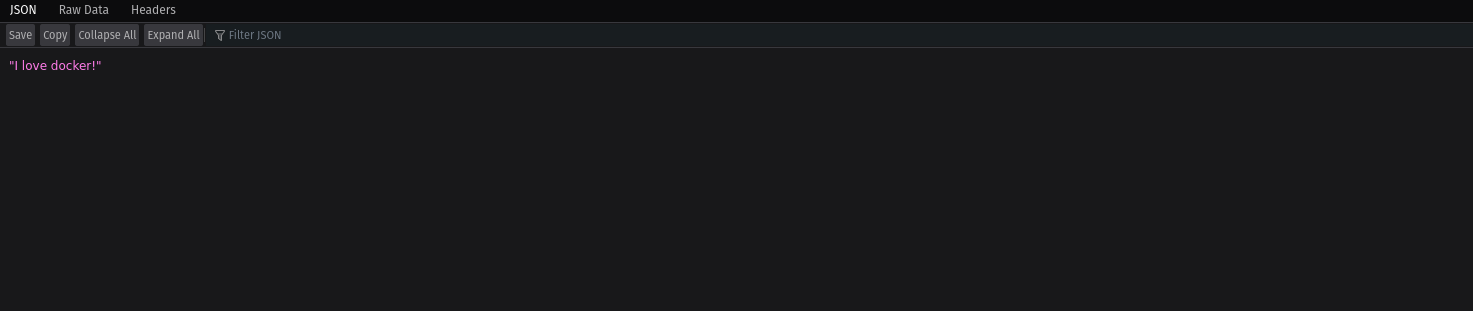
\includegraphics[scale=2.6, pagebox=artbox]{Images/server.png}
        \caption{The root route of the backend running}
        \label{fig:backend}
    \end{figure}
    \newpage
    }

    % Page 4
    \section{Exporting to docker}{
    The next step was to export the image to docker locally, to ensure the setup was
    running before deploying the automation of the Docker image to the TravisCI servers. To build a Docker image, I had to create
    a Dockerfile specifying the steps that needed to be taken to deploy the Express backend in a Docker container. The Dockerfile
    is shown in \textbf{Figure \ref{fig:dockerfile}}.
    \begin{figure}[!h]
        \centering
        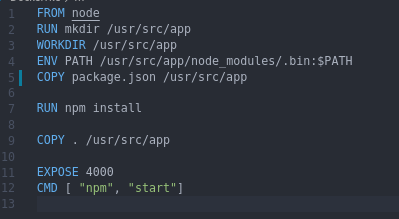
\includegraphics[scale=3, pagebox=artbox]{Images/Dockerfile.png}
        \caption{The dockerfile containing the instructions for building the container}
        \label{fig:dockerfile}
    \end{figure}
    \newline
    To prevent any unnecessary files being transferred to the Docker container, a \textbf{.dockerignore} file is defined as shown in 
    \textbf{Figure \ref{fig:dockerignore}}.
    \begin{figure}[!h]
        \centering
        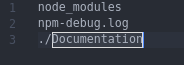
\includegraphics[scale=3, pagebox=artbox]{Images/dockerignore.png}
        \caption{The ignored files and folders when building the Docker container}
        \label{fig:dockerignore}
    \end{figure}
    \newline
    We ignored the Node Modules folder and the debug log from the Node Package Manager, thus reducing the total size of 
    the container. Now we could build the image with following command (assuming you are in the root folder of the repository):
    \begin{lstlisting}[language=bash]
        $ docker build . -t [domain]/[name]
        $ docker run -p [local port]:[docker port] 
        -d [domain]/[name]
    \end{lstlisting}
    }    
    \newpage

    % Page 5
    \section{Configuring TravisCI}
    {Before continuing, we have to create the repository, on the homepage of GitHub go to the left hand panel and click on "New". 
    This button sends you to the page seen in \textbf{Figure \ref{fig:github}}.
    \begin{figure}[!h]
        \centering
        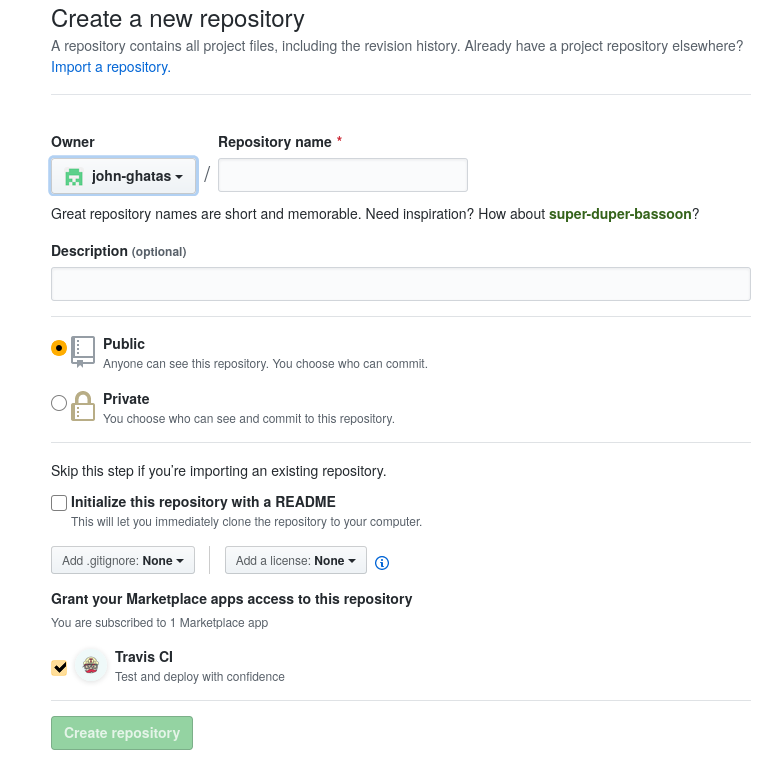
\includegraphics[scale=1.4, pagebox=artbox]{Images/github.png}
        \caption{The configuration of the GitHub repository when created}
        \label{fig:github}
    \end{figure}        
    \newline
    Fill in the repository name, keep the repository on \textbf{public} because Travis will be on a limited plan otherwise. 
    Make sure the Travis CI box is checked, and init the repo with a README if you prefer to do so. 
    \newpage
    }

    % Page 6
    \subsection{Deploying TravisCI}
    {Now that I ensured the backend runs locally, we were ready to automate the building 
    of the docker image on Travis. To configure Travis, a \textbf{.travis.yml} file was created to specify the instructions 
    for the CI tool. In \textbf{Figure \ref{fig:travis}} the configuration is shown of the travis file.
    \begin{figure}[!h]
        \centering
        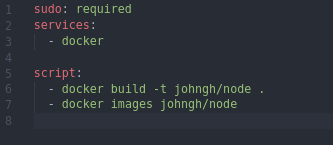
\includegraphics[scale=3, pagebox=artbox]{Images/travis.png}
        \caption{The configuration file of for the CI tool}
        \label{fig:travis}
    \end{figure}
    \newline
    The configuration file will be picked by the plugin TravisCI, that I installed on the repository automating the build. After
    the build is done the status will be updated in the README of the repository as can be seen in \textbf{Figure \ref{fig:result}}.
    \begin{figure}[!h]
        \centering
        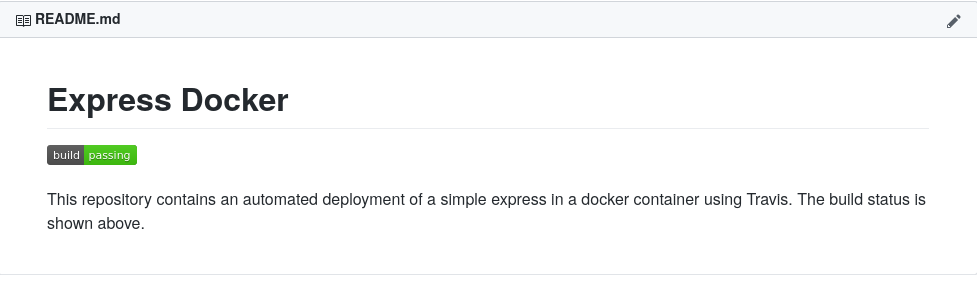
\includegraphics[scale=1.4, pagebox=artbox]{Images/README.png}
        \caption{The build status of the build of the Docker container}
        \label{fig:result}
    \end{figure}
    \newpage
    \subsection{Adding the indicator}
    {As seen in \textbf{Figure \ref{fig:result}} and indicator of the build status was added indicating whether
    the build of the Docker container passed or not. To get this container I had to login to my GitHub account linked to TravisCI
    at the \href{https://travis-ci.com/}{portal}, after which I could see my projects linked to my GitHub shown in 
    \textbf{Figure \ref{fig:travisportal}}.

    \begin{figure}[H]
        \centering
        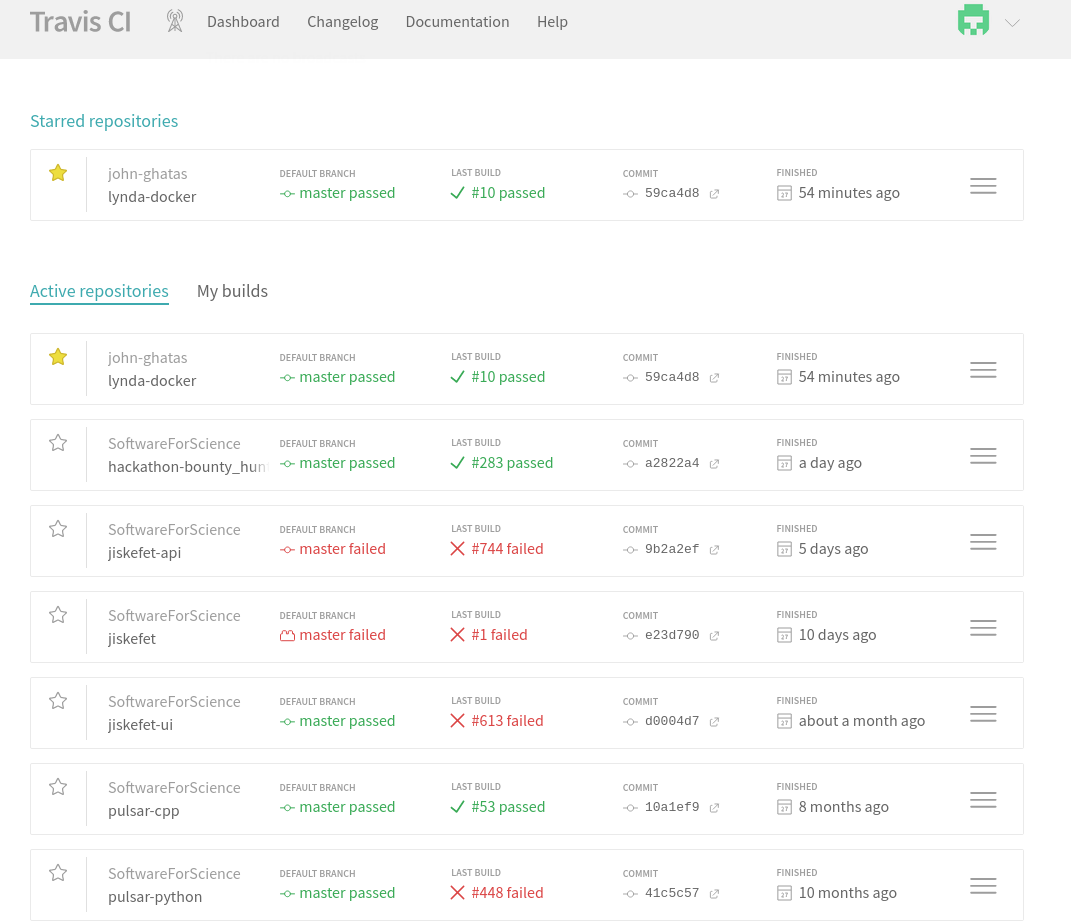
\includegraphics[scale=1.2, pagebox=artbox]{Images/travisportal.png}
        \caption{The portal with projects linked to my GitHub repositories}
        \label{fig:travisportal}
    \end{figure}
    \noindent The project I configured for building the docker container is called "lynda-docker" which I favourited in the screenshot in
    \textbf{Figure \ref{fig:travisportal}}. When I click on the project I see the status of the build in the header as  shown 
    in \textbf{Figure \ref{fig:travisstatus}}.
    \begin{figure}[H]
        \centering
        
\includegraphics[scale=1.2, pagebox=artbox]{Images/travisheader.png}
        \caption{The status of the project deploying Docker containers}
        \label{fig:travisstatus}
    \end{figure}
    \newpage
    \noindent Click on the build status, and you are presented with a screen options to embed the status. 
    The default option an Image URL as seen in \textbf{Figure \ref{fig:travisembed}}, click on the format and change it to
    Markdown, copy the result into the README.MD of the repo and the build status is embedded.
    \begin{figure}[H]
        \centering
        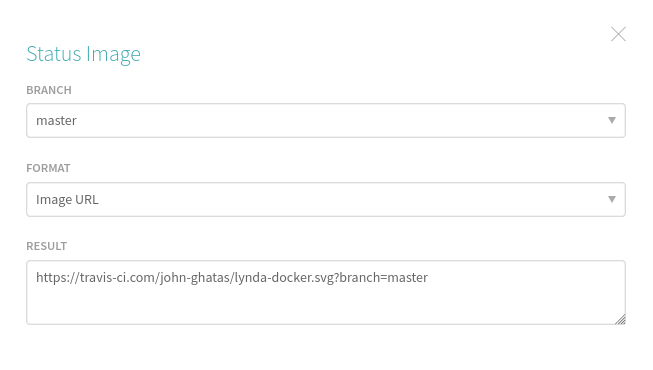
\includegraphics[scale=2, pagebox=artbox]{Images/travisembed.png}
        \caption{The embed options for the result}
        \label{fig:travisembed}
    \end{figure}

    }

\end{document}